\section{Results}
\label{sec:results}

\info{This is not finished and is just a placeholder for now.}
\pgfplotsset{width=10cm,compat=1.9}
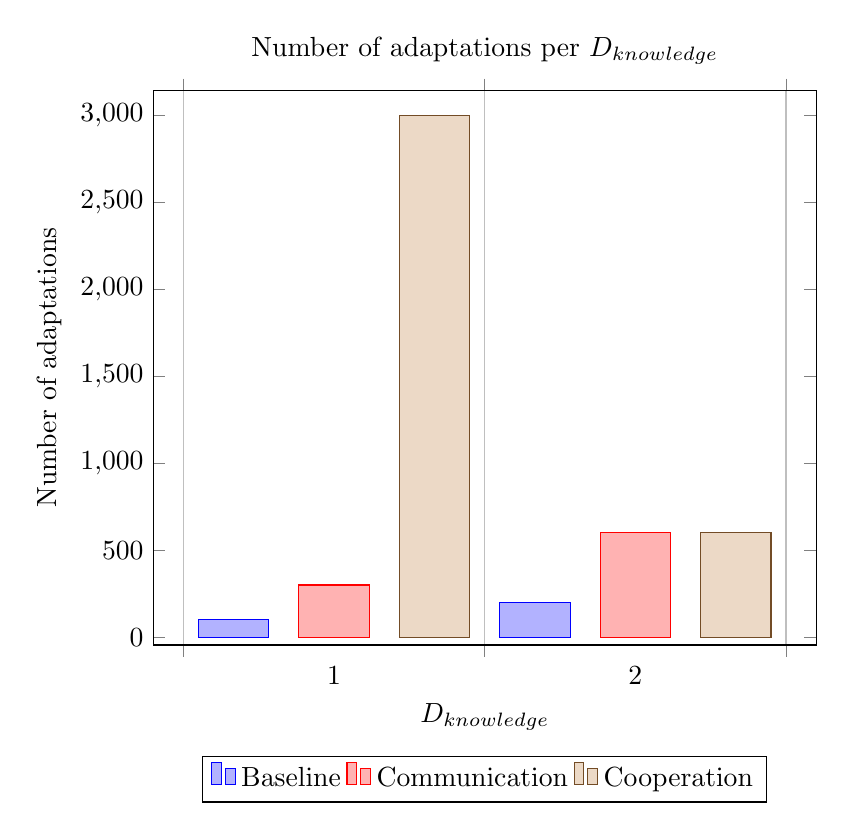
\begin{tikzpicture}
\begin{axis}[
    title={Number of adaptations per \(D_{knowledge}\)},
    x tick label style={
        /pgf/number format/1000 sep=},
    xlabel={\(D_{knowledge}\)},
    ylabel={Number of adaptations},
    enlargelimits=0.05,
    legend style={at={(0.5,-0.2)},
    anchor=north,legend columns=-1},
    ybar interval=0.7,
]
\addplot coordinates {(1,100) (2,200) (3,300)};
\addplot coordinates {(1,300) (2,600) (3,900)};
\addplot coordinates {(1,3000) (2,600) (3,900)};

\legend {Baseline, Communication, Cooperation}
\end{axis}
\end{tikzpicture}
